\documentclass[solution, letterpaper]{cs121}

\usepackage{graphicx}

%% Please fill in your name and collaboration statement here.
%\newcommand{\studentName}{Renzo Lucioni and Daniel Broudy}
%\newcommand{\collaborationStatement}{I collaborated with...}
\newcommand{\solncolor}{red}
\begin{document}

\header{2}{April 4, 2013, at 11:40 AM}{}{}

%%%%%%%%%%%%%%%%%%%%%%%%%%%%%%%%%%%%%%%%%%%%%%%%%%%%
\section*{Analytical Approach}

\hspace{4mm} The conventional algorithm requires $n^3$ multiplications and $n^2(n-1)$ additions. Thus, the work required by the conventional algorithm, used when $n \leq n_0$, is $n^3 + n^2(n-1) = 2n^3 - n^2$. Strassen's algorithm requires 7 matrix products per recurrence, 10 additions and subtractions when deriving the $P_1, \ldots, P_7$, and 8 additions and subtractions when manipulating the $P_i$'s to find the matrix sums. The work required by Strassen's algorithm, used when $n > n_0$, can be represented by the recurrence $T(n) = 7T(\frac{n}{2}) + (10+8)\frac{n^2}{4} = 7T(\frac{n}{2}) + \frac{9}{2}n^2$, where $T(1) = 1$.

To determine the ideal crossover point analytically we find the location at which changing to Strassen's first starts to provide a benefit in runtime (i.e., the first point at which $T(n)$ for Strassen's is less than $T(n)$ for the conventional method). In order to find this location, we define a recurrence for Strassen's featuring the crossover as follows:
\[
\begin{array}{rcl}
T(n) &=& 7T(\frac{n}{2}) + \frac{9}{2}n^2\\
&=& 7(2(\frac{n}{2})^3 - (\frac{n}{2})^2) + \frac{9}{2}n^2\\
&=& 7(2\frac{n^3}{4} - \frac{n^2}{4}) + \frac{9}{2}n^2\\
&=& 14\frac{n^3}{4} - 7\frac{n^2}{4} + \frac{9}{2}n^2\\
&=& \frac{7n^3}{2} - \frac{11n^2}{2}\\
\end{array}
\]

We can then compare this to the conventional method and determine at which point switching to Strassen's begins to benefit the running time, since the above recurrence is the recurrence containing one call to Strassen's. We set $\frac{7n^3}{2} - \frac{11n^2}{2}$ equal to $2n^3 - n^2$ and achieve an intersection at 15. Thus, Strassen's becomes effective when $n = 15$. When $n=15$ with one call to Strassen's, the crossover point is 7.5. However, because it does not make sense to crossover at 7.5, we round the crossover point up to 8. If we had rounded down to 7 then Strassen's should have become effective at $n = 14$. Thus, we have analytically determined that the crossover should be 8; that is, $n_0 = 8$.

\section*{Experimental Approach}

\hspace{4mm}We first implemented the conventional algorithm for matrix multiplication. We then implemented Strassen's algorithm for matrices where $n$ is a power of 2. We extended this implementation for more general values of $n$ by padding the initial matrices with $N - n$  0's where $N$ is the closest power of 2 greater than or equal to $n$, as suggested in the hints section of the spec. We tied the two algorithms together by adding a conditional to our implementation of Strassen's to check whether or not the current dimension is less than or equal to some crossover value $n_0$. If so, computation switches to our implementation of the conventional algorithm from within Strassen's algorithm. 

We tested for the optimal value of $n_0$ by running our modified version of Strassen's algorithm on matrices where $n=500$ and $n=1000$. In these matrices, every element was randomly selected to be 0, 1, or 2. The graphs below illustrate our results, plotting the computation time associated with each possible value of $n_0$, averaged over 45 and 15 runs for $n=500$ and $n=1000$, respectively.

\begin{center}
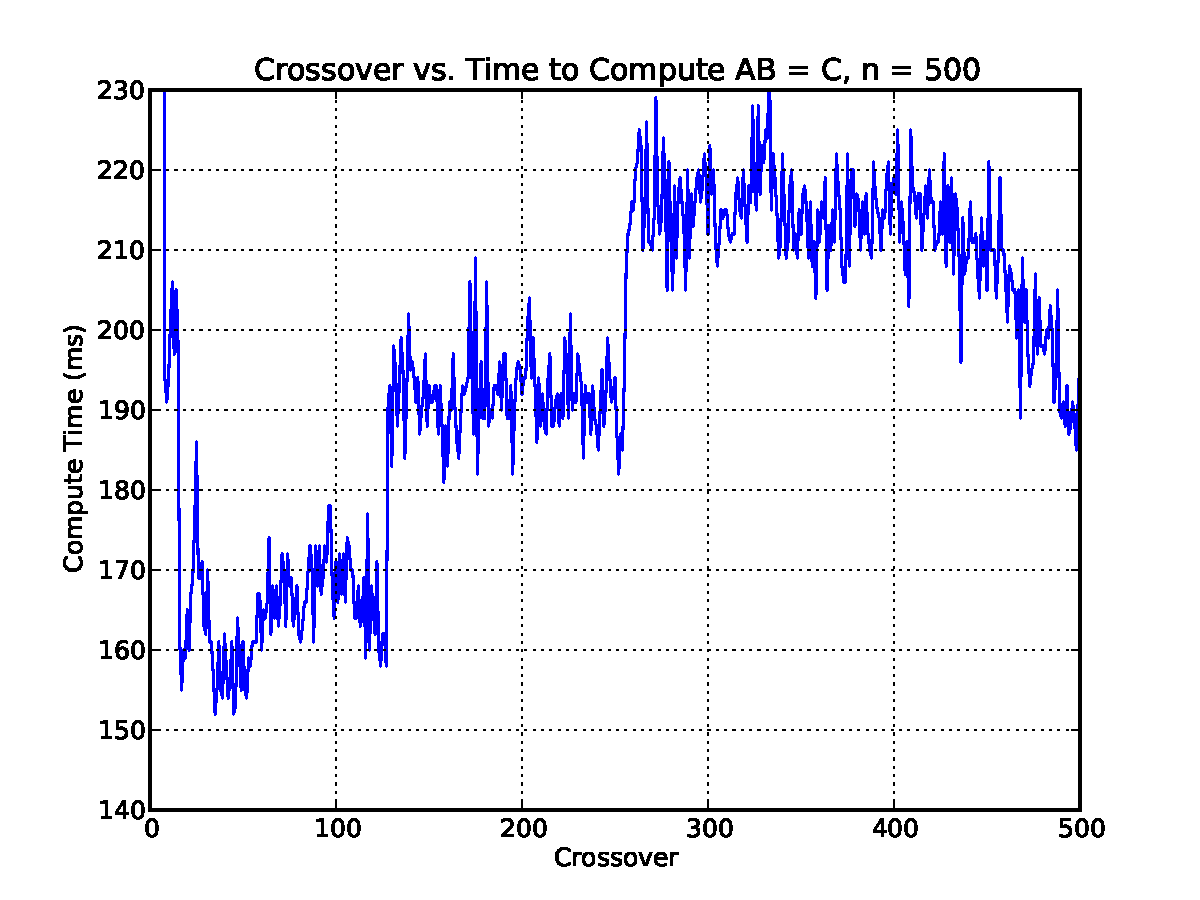
\includegraphics[scale=0.72]{crossover-v-compute-time-500-msec.pdf}
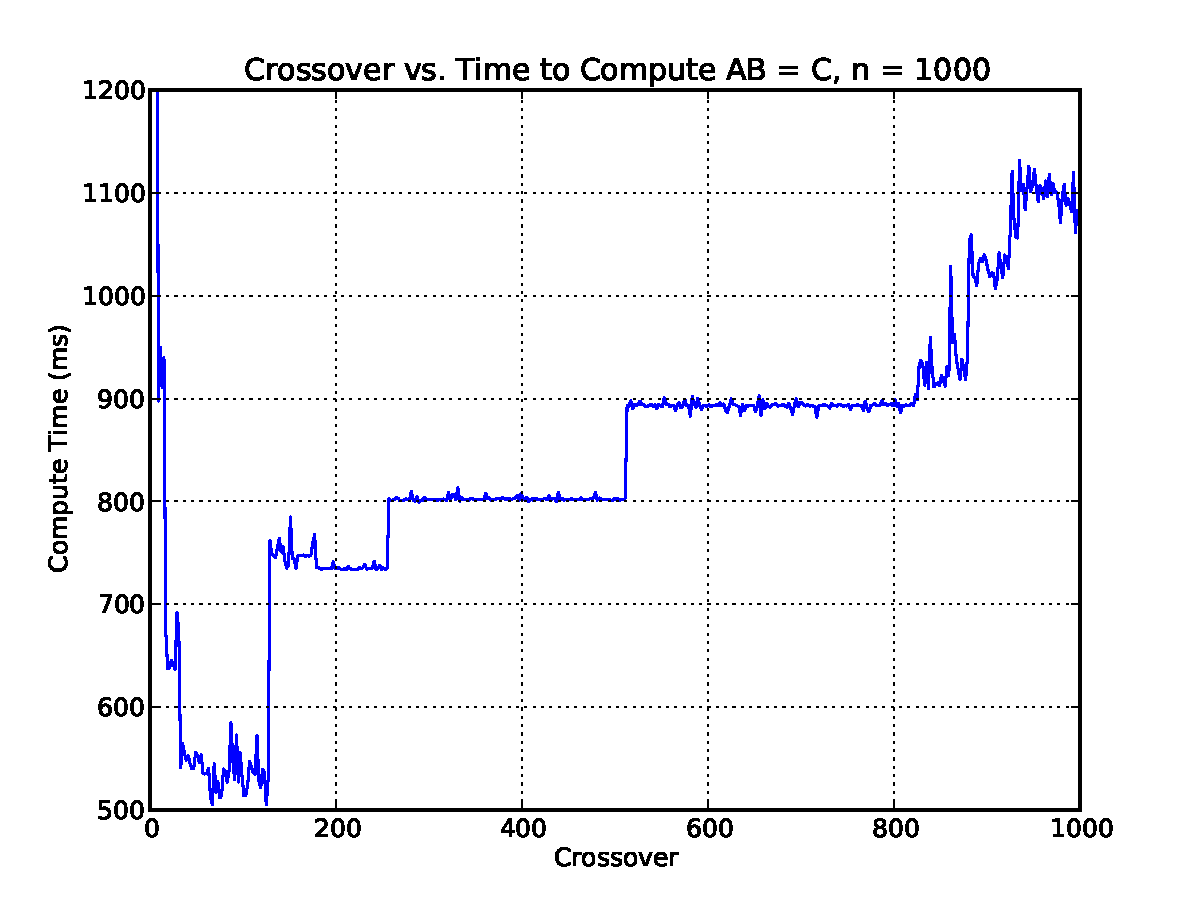
\includegraphics[scale=0.72]{crossover-v-compute-time-1000-msec.pdf}
\end{center}

The most prominent feature of these graphs is their stepped pattern. This results from the fact that Strassen's operates on matrices for which $n$ is a power of 2 - the initial padding for all other matrices guarantees this. In each recursive call to Strassen's, $n$ is cut in half. Consequently, for all $n_0$ in a range of the form $[2^m, 2^{m+1})$, the crossover will take effect after the same number of calls to Strassen's algorithm, and thus the running time is expected to behave the same. To see this, consider the case in which $n$ is initially 64. For any value of $n_0$ in the range $[32,64)$, Strassen's will execute once before control is passed to the conventional algorithm. After one iteration of Strassen's, $n= 32$, and thus all previously mentioned crossover points would have taken effect. Note that this logic also explains why the steps occur at powers of 2.

Each step indicates the time (in milliseconds) required to multiply two matrices of the indicated size. In the graph where $n=500$, our minimum compute time, 83.67 ms, occurs at a crossover of 114. Because of the above logic - $n_0$ in the range $[2^m,2^{m+1})$ behave the same - this is equivalent to a crossover point of 64. The larger value of $n$ provides us with a much clearer picture. This is due partially to the longer runtimes, which minimize the effect of small variations in runtime. In the graph where $n=1000$, our minimum compute time, 505.07 ms, occurs at a crossover of 125. The second shortest time for $n = 1000$ is 505.27 ms and occurs at $n_0 = 65$. These two minimums almost perfectly demarcate the step that occurs on the range [64, 128). It is worth noting that this step is rather jagged due to the small times being plotted; as mentioned, larger times would minimize the effect of these small variations. In both graphs, the lowest step begins near a crossover value of 64, leading us to conclude that in practice, $n_0 = 64$ \textit{(Note: as previously described, any value in $[64,128)$ would be appropriate)}. This crossover value is now hardcoded into our implementation as a constant; the infrastructure we used to find it is still in place, just commented out.

\section*{Discussion}

\subsection*{Crossover Point}
\hspace{4mm} The lowest crossover point we could decide on was $n_0 = 64$, as discussed above. While all arithmetic operations are assumed to be cost 1 in the analytical approximation of the crossover point, in reality these operations have distinct values. Furthermore, some operations were assumed to be free in the analytical approach, explaining the discrepancy between the analytically and experimentally determined crossover values.

\subsection*{Difficulties}
\hspace{4mm} Several difficulties arose when implementing Strassen's. The most pressing of these challenges was how to properly utilize and re-use memory. That said, this is an optimization issue, and so we will hold off on discussion of this topic until the next subsection. We also struggled to properly index into our original matrices in order to work in place. Using standard debugging techniques such as print statements, we were able to solve this problem relatively quickly.

\subsection*{Optimization}
\hspace{4mm} We optimized our implementation of the conventional algorithm by taking locality of reference into consideration in our three {\tt for} loops.

We applied several optimizations to our implementation of Strassen's. First, we worked to re-use memory whenever possible to minimize the number of system calls like \texttt{malloc} and \texttt{free}. We did this by allocating the necessary space for all matrices $P$ from Strassen's algorithm and then one more for workspace. Using this method and being cautious about memory usage, we were able to limit ourselves to one call to \texttt{malloc} and one call to \texttt{free} in each call to Strassen's. Note that while it might be possible to further optimize and use only one \texttt{malloc} and \texttt{free} for the entire algorithm, we decided that the number of calls was small enough to make this difference negligible on the whole. The implementation of the technique we did use was not trivial and required the creation of a matrix struct to store the metadata allowing us to locate each sub-matrix within the original matrix. Originally, we worked with \texttt{matrix} structs, passing them around by pointer, but this hurt cache line optimization. Because only the contained array is of significant size and it is stored via reference, we were able to work with \texttt{matrix} structs without the use of pointers.

In addition, we optimized the calculation of AE + BG and CF + DH in Strassen's by creating special functions that simultaneously perform all the necessary additions and subtractions, thereby avoid multiple passthroughs.

Finally, we optimized the calculation of the necessary padding using a bit manipulation technique described here: http://graphics.stanford.edu/~seander/bithacks.html. We added a conditional to this technique to allow the code to work on both 32 and 64-bit architectures (assuming it is compiled on each architecture separately).

\subsection*{Timing}
\hspace{4mm} We defined the runtime of our implementation of the modified Strassen's algorithm as the number of clock cycles elapsed while the multiplication algorithm was running on the CPU. That is, we used CPU time as our definition of time. Note that this does not include the time required to pad matrices, if necessary, or print the diagonal elements of the final matrix. Although important to the total runtime of our program, these steps do not figure into finding the optimal crossover point because they are not part of then matrix multiplication step.

\subsection*{Largest $n$}
\hspace{4mm} The largest value of $n$ we tested our program on was $n = 10000$; we were able to successfully multiply these matrices.

\subsection*{Matrix Type}
\hspace{4mm} In our implementation, we chose to multiply {\tt int}'s, specifically {\tt int32\_t}'s (to be consistent across architectures), but this choice does not matter. We could just as easily swap them out for floats, and the program would function as expected.

\end{document}



